\nomenclature[]{DBN}{Dynamic Bayesian Network}
\nomenclature[]{BN}{Bayesian Network}
\nomenclature[]{CPD}{Conditional Probability Distribution}
\nomenclature[]{2TDBN}{2 Time Slice Dynamic Bayesian Network}

Dynamic Bayesian Networks are a generalization of HMMs and are used to model time series, without being limited to the assumptions of HMMs. The key difference between DBNs and HMMs is that DBNs are not limited in how they decompose the state of a complex stochastic system into the variables that represent its constituent distributions \cite{AIAMA}. Technically, every DBN can be represented as a HMM and visa versa, however, the number of parameters that need to be detemined to represent DBNs can be significantly less that that of HMMs. This is due to the fact that specifying a full joint discrete distribution can require an exponential number of probabilities, whereas specifying the same joint distribution as factored conditional distributions may require far fewer.

\subsubsection{A Note on Bayesian Networks}
A Bayesian Network (BN) is a graphical way to represent a particular factorization of a joint distribution. For a detailed explanation, the reader is referred to \cite{KollerPGM}. To fully explain a complex system, it is often natural to model it as the joint distribution of a number of random variables. This is in general intractable \cite{KollerPGM}. In order to circumvent this, independence properties in the distribution can be exploited to provide a much more compact representation of the distribution. BNs exploit the fact that independence is a strong notion that doesn't often occur in the real-world; however conditional independence is a weaker property that is far more prevalent, which still leads to the desired compact representation. BNs are described by a directed acyclic graph (DAG), $G$. The nodes in the graph correspond to the random variables whose joint distribution is of interest, and the arcs represent conditional independences. Specifically, if one Burglary points to Alarm as in figure \ref{fig:BayesianNetwork}, it is implied that the distribution of Alarm is conditionally independent on all other nodes in the network given Burglary. This means that only a local conditional probability distribution must be provided in order to specify the full joint distribution.

\begin{figure}
%example bayesian network figure
\begin{tikzpicture}[
  node distance=1cm and 0cm,
  mynode/.style={draw,ellipse,text width=2cm,align=center}
]
\node[mynode] (i) {Burglary};
\node[mynode,below right=of i] (g) {Alarm};
\node[mynode,above right=of g] (c) {Earthquake};
\path %(ra) edge[latex-] (sp)
(g) edge[latex-] (c) 
(g) edge[latex-] (i);
\node[left=0.5cm of i]
{
\begin{tabular}{cM{2}M{2}}
\toprule
\multicolumn{2}{c}{Burglary} \\
\multicolumn{1}{c}{T} & \multicolumn{1}{c}{F} \\
\cmidrule(r){1-2}
0.001 & 0.999 \\
\bottomrule
\end{tabular}
};
\node[right=0.5cm of c]
{
\begin{tabular}{cM{2}M{2}}
\toprule
\multicolumn{2}{c}{Earthquake} \\
\multicolumn{1}{c}{T} & \multicolumn{1}{c}{F} \\
\cmidrule(r){1-2}
0.008 & 0.992 \\
\bottomrule
\end{tabular}
};
\node[below=0.5cm of g]
{
\begin{tabular}{ccM{2}M{2}}
\toprule
& & \multicolumn{2}{c}{Alarm} \\
\multicolumn{2}{l}{Burglary Earthquake} & \multicolumn{1}{c}{T} & \multicolumn{1}{c}{F} \\
\cmidrule(r){1-2}\cmidrule(l){3-4}
F & F & 0.01 & 0.99 \\
F & T & 0.95 & 0.05 \\
T & F & 0.8 & 0.2 \\
T & T & 0.99 & 0.01 \\
\bottomrule
\end{tabular}
};
\end{tikzpicture}

\caption{Simple Bayesian Network based on \cite[P.~512]{AIAMA}}
\label{fig:BayesianNetwork}
\end{figure}







\subsubsection{Dynamic Bayesian Network Description}
A Dynamic Bayesian Network is a Bayesian Network that represents a general temporal probability model that describes a random system which is assumed to have a number of random variables, some of which are observable and some not. \cite{AIAMA}. Dynamic Bayesian networks are usually used to represent the dynamics of a random system over time and can be described generally by specifying how the system transitions from its state at t-1 to t, if the first order Markov property is assumed. It is often convenient to categorise the random variables in the network into state variables, assumed to be hidden, control variables and observation variables \note{might be better to change the names of these}. An example of a Dynamic Bayesian Network can be seen in figure \ref{fig:2TDBNExample}. The hidden state variables are shaded in light grey, the observation variables in light orange (saffron), the control variables in light green. The arrows indicate conditional indepences, as with regular Bayesian Networks.

\begin{figure}
    \centering
    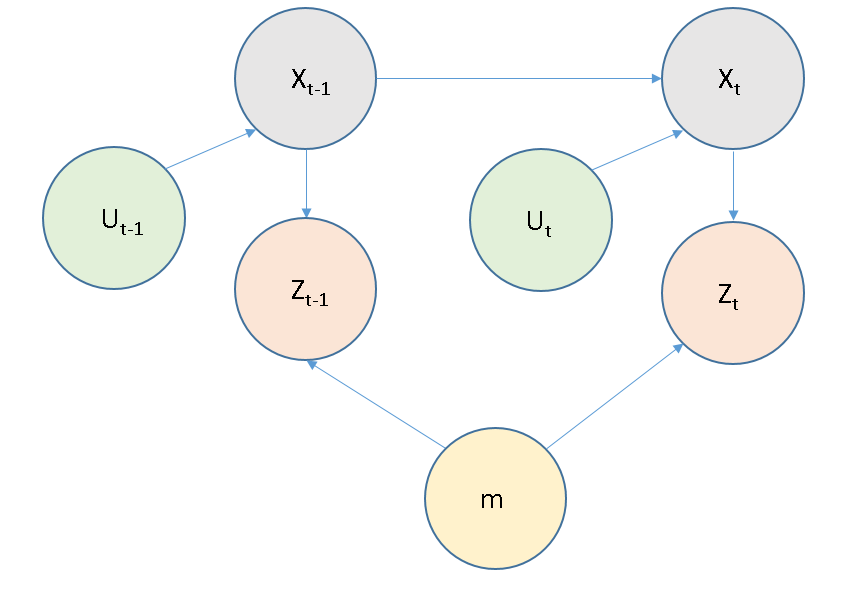
\includegraphics[width = 0.5\linewidth]{Chapters/MultiAgentTargetDetection/BayesianFiltering/Figs/DBNs/2DBNExample.png}
    \caption{A DBN used for \textbf{S}imulatenous \textbf{L}ocalisation \textbf{A}nd \textbf{M}apping (SLAM), based on \cite[p.~311]{Thrun:2005:ProbabilisticRobotics}}
    \label{fig:2TDBNExample}
\end{figure}


\subsubsection{}